% Insert after the main performance table; not a standalone document.
\subsection{Paired Sensitivity to Visual-Language Changes}
We hold the question, reference answer, and optional source context fixed in English or Chinese and vary the visual language across 24 versions of each seed. The corresponding same-language visual provides the baseline. We report the mean accuracy difference and both directions of correctness flips, using all $128\times23$ cross-language pairs as the denominator for each question language. Confidence intervals resample the 128 seeds with all their language variants, using 10,000 bootstrap draws.

% Requires booktabs and multirow. Semantic ACC; each seed is a bootstrap cluster.
\begin{table*}[t]
\centering
\scriptsize
\begin{tabular*}{\textwidth}{@{\extracolsep{\fill}}lrrrrrrrr@{}}
\toprule
\multirow{2}{*}{Model} & \multicolumn{2}{c}{Charts $\Delta$ACC} & \multicolumn{2}{c}{Tables $\Delta$ACC} & \multicolumn{2}{c}{Correct$\to$Wrong} & \multicolumn{2}{c}{Wrong$\to$Correct} \\
\cmidrule(lr){2-3}\cmidrule(lr){4-5}\cmidrule(lr){6-7}\cmidrule(lr){8-9}
& EN & ZH & EN & ZH & EN & ZH & EN & ZH \\
\midrule
GPT-6 Astra & -2.7 & -2.2 & -7.4 & -10.3 & 4.5 & 6.4 & 0.3 & 1.6 \\
Gemini-3.8-Flash & -1.2 & +1.3 & -2.2 & -3.0 & 3.2 & 2.9 & 1.7 & 2.9 \\
GPT-5.6-Sol & -2.2 & -1.4 & -3.3 & -3.9 & 4.4 & 6.2 & 1.9 & 4.0 \\
GPT-5.6-Luna & -4.4 & -0.9 & -10.5 & +0.3 & 8.5 & 6.4 & 2.1 & 5.8 \\
\bottomrule
\end{tabular*}
\caption{Paired sensitivity to visual-language changes. Questions and answers remain in EN or ZH. $\Delta$ACC (percentage points) compares the other 23 visual languages with the same-language baseline, separately for charts ($n=87$) and tables ($n=41$). Both flip rates use all $128\times23$ pairs as their denominator (\%). Failures retain the main-table scoring policy.}
\label{tab:paired-language-sensitivity}
\end{table*}

Average accuracy can conceal opposing changes at the instance level. For Gemini-3.8-Flash with Chinese questions, the net change is only $-0.03$ percentage points, yet 2.92\% of pairs change from correct to wrong and 2.89\% change from wrong to correct. GPT-5.6-Luna shows a similar cancellation: a net change of $-0.54$ points comprises 6.39\% correct-to-wrong and 5.84\% wrong-to-correct flips. GPT-6 Astra instead exhibits a net decline for both English ($-4.21$ points; 95\% CI $[-7.13,-1.83]$) and Chinese ($-4.82$; $[-9.04,-0.92]$). These are descriptive comparisons of visual-language versions, which can differ in font and layout as well as text; they do not isolate OCR or language understanding.

The correct-coverage curves further distinguish average performance from reliability across languages. With English questions, the fraction of seeds answered correctly in all 24 visual languages is 70.3\% for GPT-6 Astra and Gemini-3.8-Flash, 57.0\% for GPT-5.6-Sol, and 39.1\% for GPT-5.6-Luna. The corresponding Chinese values are 67.2\%, 64.8\%, 49.2\%, and 42.2\%. Each configuration was evaluated once: these curves include generation and judging variability and do not estimate test--retest reliability.

All analyses reuse the frozen main-table predictions and judgments, including the original treatment of failed requests. No configurations are repaired, rerun, or excluded. Nominal prompts are verified across all variants; historical generation-setting changes and format-only fallback are retained, and some legacy attempts lack effective-prompt hashes. The results therefore describe paired sensitivity under the recorded evaluation protocol, rather than a perfectly uniform historical inference protocol.

% Upload outputs/paired_analysis/cross_language_coverage.pdf to Overleaf img/.
\begin{figure*}[t]
\centering
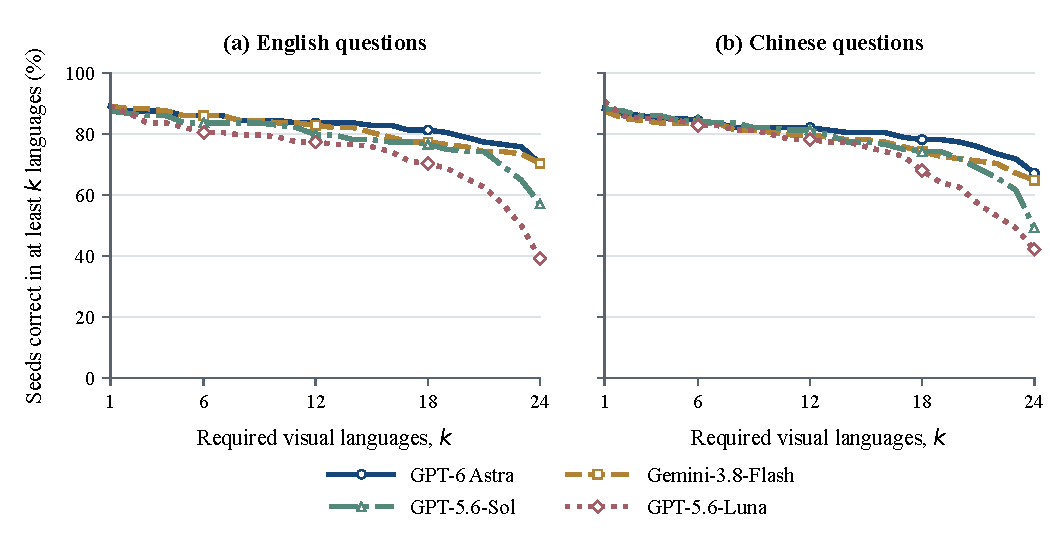
\includegraphics[width=\textwidth]{img/cross_language_coverage.pdf}
\caption{Cross-language correct coverage for fixed English (left) and Chinese (right) questions and answers. At threshold $k$, the ordinate is the percentage of 128 seeds answered correctly in at least $k$ of the 24 visual languages. The right endpoint requires every visual-language variant to be correct.}
\label{fig:cross-language-coverage}
\end{figure*}
